\documentclass[a4paper,oneside,12pt]{article}
\usepackage{mystyle}

\title{\Large\bf Periodic Batching\footnote{%%
    Updated by quacksouls, \url{https://github.com/quacksouls}
  }}
\author{%%
  stalefishies \\
  \url{https://github.com/stalefishies}
}
\date{\today}

\begin{document}

\maketitle

\noindent
A fundamental problem in scheduling HWGW batching is to ensure scripts
never start at a raised security level.  Here, we solve the problem
with a batch schedule that is \emph{periodic}.  By leaving a carefully
calculated safe window between each HWGW, we can ensure that all
hacks, grows, and weakens start in that window and so begin at minimum
security.  This periodic schedule can then be repeated as long as it
remains valid -- in theory forever, but in practice until the hacking
level increases, though we describe a way of mitigating this
limitation at the end.

First, we define a timing model, which tells us the structure of the
batches we want to achieve.  As usual, we need to leave some time
buffer between events to work with JavaScript concurrency timing.  We
call that time $t_0$.  The timing model we will use is illustrated in
\Figure{fig:batching_model}.

\begin{figure}[!htbp]
\centering
\captionsetup{font=normal,justification=justified}
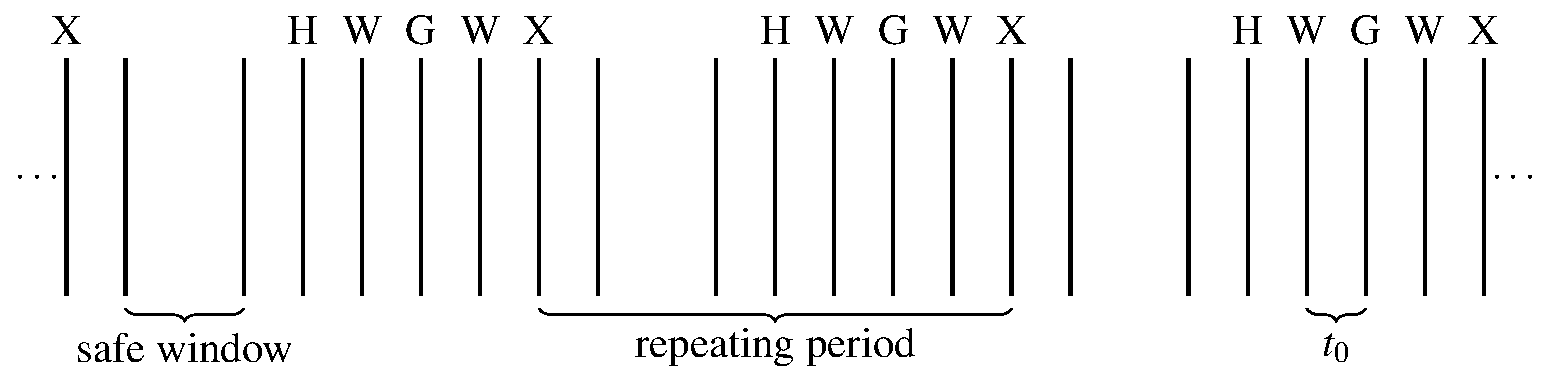
\includegraphics[scale=0.525]{image/model.pdf}
\caption{%%
  A timing model for batching.
}
\label{fig:batching_model}
\end{figure}

%% H, G, and W respectively denote when hacks, grows, and weakens end, and X denotes a point where a batch manager script both checks the previous batch completed properly and also launches scripts for the next batch. Different timing windows are possible: for example, you may want to run HGW batching, or have your manager script run at a different point, or use different buffer times between different events. Ideally, these notes should let you work through the calculations required to calculate a schedule for any timing model.

%% Before moving on those calculations, first we show two sketches to help visualise the timing model we're using here. First, we show an example of a HWGW batch where each script overlaps with 10 different periods:
%% \begin{diagram}[x = 0.13ex, y = 1.3ex]
%%   \foreach \i in {0, ..., 9} {
%%   \foreach \j in {0, 10, 34, 44, 54, 64, 74} {
%%   \draw (84 * \i + \j, 0) to +(0, 5);
%% }
%% }
%%   \draw (840, 0) to +(0, 5);

%%   \node at (  0, 5) [above] {\clap{\tiny X}};
%%   \node at (800, 5) [above] {\clap{\tiny H}};
%%   \node at (810, 5) [above] {\clap{\tiny W}};
%%   \node at (820, 5) [above] {\clap{\tiny G}};
%%   \node at (830, 5) [above] {\clap{\tiny W}};
%%   \node at (840, 5) [above] {\clap{\tiny X}};

%%   \draw [dotted] (0, 4) to (600, 4);
%%   \draw (600, 4) to (800, 4);
%%   \draw [dotted] (0, 3) to (10, 3);
%%   \draw (10, 3) to (810, 3);
%%   \draw [dotted] (0, 2) to (180, 2);
%%   \draw (180, 2) to (820, 2);
%%   \draw [dotted] (0, 1) to (30, 1);
%%   \draw (30, 1) to (830, 1);

%%   \draw [decorate, decoration = {brace, mirror}] ( 10, -0.5) to
%%   node [below, midway] {\clap{\scriptsize Weakens begin}} ( 34, -0.5);
%%   \draw [decorate, decoration = {brace, mirror}] (178, -0.5) to
%%   node [below, midway] {\clap{\scriptsize Grow begins}}   (202, -0.5);
%%   \draw [decorate, decoration = {brace, mirror}] (598, -0.5) to
%%   node [below, midway] {\clap{\scriptsize Hack begins}}   (622, -0.5);
%% \end{diagram}
%% The dotted lines denotes the time each script is sleeping, and the solid lines denote the actual duration of the hack, grow, or weaken. Since each script overlaps with $10$ periods, we can run $10$ batches simultaneously; all $10$ simultaneous batches are depicted below, each offset by a different number of periods:
%% \begin{diagram}[x = 0.13ex, y = 0.75ex]
%%   \foreach \i in {0, ..., 9} {
%%   \foreach \j in {0, 10, 34, 44, 54, 64, 74} {
%%   \draw (84 * \i + \j, 1) to +(0, 61);
%% }
%% }
%%   \draw (840, 1) to +(0, 61);

%%   \foreach \i in {0, ..., 8} {
%%   \draw [dotted] (\i * 84 + 84, 60 - 6 * \i) to ({min(\i * 84 + 684, 840)}, 60 - 6 * \i);
%%   \draw ({min(\i * 84 + 684, 840)}, 60 - 6 * \i) to (840, 60 - 6 * \i);
%%   \draw [dotted] (\i * 84 + 84, 59 - 6 * \i) to ({min(\i * 84 +  94, 840)}, 59 - 6 * \i);
%%   \draw ({min(\i * 84 +  94, 840)}, 59 - 6 * \i) to (840, 59 - 6 * \i);
%%   \draw [dotted] (\i * 84 + 84, 58 - 6 * \i) to ({min(\i * 84 + 264, 840)}, 58 - 6 * \i);
%%   \draw ({min(\i * 84 + 264, 840)}, 58 - 6 * \i) to (840, 58 - 6 * \i);
%%   \draw [dotted] (\i * 84 + 84, 57 - 6 * \i) to ({min(\i * 84 + 114, 840)}, 57 - 6 * \i);
%%   \draw ({min(\i * 84 + 114, 840)}, 57 - 6 * \i) to (840, 57 - 6 * \i);
%% }

%%   \foreach \i in {0, ..., 9} {
%%   \draw [dotted] (0, 60 - 6 * \i) to ({max(0, \i * 84 - 156)}, 60 - 6 * \i);
%%   \draw ({max(0, \i * 84 - 156)}, 60 - 6 * \i) to (84 * \i + 44, 60 - 6 * \i);
%%   \draw [dotted] (0, 59 - 6 * \i) to ({max(0, \i * 84 - 746)}, 59 - 6 * \i);
%%   \draw ({max(0, \i * 84 - 746)}, 59 - 6 * \i) to (84 * \i + 54, 59 - 6 * \i);
%%   \draw [dotted] (0, 58 - 6 * \i) to ({max(0, \i * 84 - 576)}, 58 - 6 * \i);
%%   \draw ({max(0, \i * 84 - 576)}, 58 - 6 * \i) to (84 * \i + 64, 58 - 6 * \i);
%%   \draw [dotted] (0, 57 - 6 * \i) to ({max(0, \i * 84 - 726)}, 57 - 6 * \i);
%%   \draw ({max(0, \i * 84 - 726)}, 57 - 6 * \i) to (84 * \i + 74, 57 - 6 * \i);
%% }
%% \end{diagram}
%% Our goal is to calculate two values: the period, $T$, which is the time taken for the process to go through one cycle, and the depth, $k_W$, which is the number of batches we can run simultaneously. (The reason for calling the depth `$k_W$' will be clear shortly.) In particular, we want $T$ to be as small as possible, to maximise the rate of HWGW batching.

%% To do so, first imagine we have some fixed schedule, and we can vary the hack time however we wish. If we want our hack to start in the particular safe window depicted above, what possible hack times could we have? Clearly, the longest possible hack time has the hack starting at the beginning of the window, and the shortest hack time starts at the end of the window:
%% \begin{diagram}[x = 0.05cm, y = 0.5cm]
%%   \foreach \i in {0, ..., 2} {
%%   \foreach \j in {0, 10, 20, 30, 40, 50, 60} {
%%   \draw (84 * \i + \j, 0) to +(0, 3);
%% }
%% }
%%   \draw (252, 0) to +(0, 3);
%%   \draw (262, 0) to +(0, 3);
%%   \draw (272, 0) to +(0, 3);

%%   \draw [dotted] (-10, 2) to (60, 2) (-10, 1) to (84, 1);
%%   \draw (60, 2) to (262, 2) (84, 1) to (262, 1);

%%   \draw [|-|] (60,  3.5) to node [midway, fill = white, inner sep = 1pt] {Longest possible hack time}  (262,  3.5);
%%   \draw [|-|] (84, -0.5) to node [midway, fill = white, inner sep = 1pt] {Shortest possible hack time} (262, -0.5);
%% \end{diagram}
%% Of course, the hack time does not have to overlap exactly three periods. We define $k_H$ as the number of periods the hack overlaps; every hack has to occupy at least one period, so we must have $k_H \ge 1$. Given a particular $k_H$, period $T$, and buffer $t_0$, we can bound the hack time in terms of those values:
%% \begin{diagram}[x = 0.05cm, y = 0.5cm]
%%   \foreach \i in {0, ..., 2} {
%%   \foreach \j in {0, 10, 20, 30, 40, 50, 60} {
%%   \draw (84 * \i + \j, 0) to +(0, 3);
%% }
%% }
%%   \draw (252, 0) to +(0, 3);
%%   \draw (262, 0) to +(0, 3);
%%   \draw (272, 0) to +(0, 3);

%%   \draw [dotted] (-10, 2) to (60, 2) (-10, 1) to (84, 1);
%%   \draw (60, 2) to (262, 2) (84, 1) to (262, 1);

%%   \draw [|-|] (10,  3.5) to node [midway, fill = white, inner sep = 1pt] {$k_H T$}      (262,  3.5);
%%   \draw [|-|] (10,  4.0) to node [midway, fill = white, inner sep = 1pt] {$5 t_0$}      ( 60,  4.0);
%%   \draw [|-|] (94, -0.5) to node [midway, fill = white, inner sep = 1pt] {$(k_H - 1)T$} (262, -0.5);
%%   \draw [|-|] (84, -0.5) to node [midway, fill = white, inner sep = 1pt] {$t_0$}        ( 94, -0.5);
%% \end{diagram}
%% Thus, denoting the hack time as $T_H$, the hack time must be bounded by:
%% \begin{equation}
%%   \eqlabel{hack}
%%   (k_H - 1)T + t_0 \le T_H \le k_H T - 5 t_0
%% \end{equation}
%% In other words, if we choose $k_H$ and $T$ such that the above bounds hold, we are guaranteed to have the start of the hack fall in a safe window.

%% Similar analysis of grow gives rise to a parameter $k_G \ge 1$ which is used to bound the grow time, $T_G$:
%% \begin{equation}
%%   \eqlabel{grow}
%%   (k_G - 1)T + 3 t_0 \le T_G \le k_G T - 3 t_0
%% \end{equation}

%% With the weakens, we must be a little careful since there's two of them; in order for both weakens to lie within the safe window, we require the bounds:
%% \begin{equation}
%%   \eqlabel{weak}
%%   (k_W - 1)T + 4 t_0 \le T_W \le k_W T - 4 t_0
%% \end{equation}
%% Since the weaken time is always the longest, it is $k_W$ which determines how many periods the entire batch overlaps, and thus how many batches can run concurrently; hence $k_W$ is equivalent to the depth.

%% Thus, our objective is, given times $T_H$, $T_G$, $T_W$, and $t_0$, determine $k_H$, $k_G$, and $k_W$ such that the above bounds are satisfied with the minimum possible choice of $T$.

%% To actually calculate this, first note that the hack, grow, and weaken times are all defined to be directly related to each other:
%% \begin{equation}
%%   T_G = \frac{16}{5} T_H \qquad T_W = 4 T_H
%% \end{equation}
%% This lets us write down direct relations between $k_H$, $k_G$, and $k_W$. Taking half of \eqref{hack} and \eqref{weak} each:
%% \begin{equation}
%%   4 \big[ (k_H - 1)T + t_0 \big] \le T_W \qquad T_W \le k_W T - 4 t_0
%% \end{equation}
%% Combining the two inequalities and rearranging:
%% \begin{align}
     %%      4k_H T - 4T + 4 t_0 &\le k_W T - 4 t_0 \\
%%   k_H + \frac{2t_0}{T} &\le \frac14 k_W + 1 \\
     %%      \intertext{But clearly $k_H \le k_H + \frac{2t_0}{T}$. Thus, we can drop that term and simply write:}
     %%      k_H &\le \frac14 k_W + 1 \\
%%     \intertext{And since $k_H$ must be an integer, we can tighten this to:}
%%     k_H &\le \left\lfloor \frac14 k_W + 1 \right\rfloor
%% \end{align}
%% Taking the other halves of \eqref{hack} and \eqref{weak} gives:
%% \begin{equation}
%%     (k_W - 1)T + 4t_0 \le T_W \qquad T_W \le 4 \big[ k_H T - 5 t_0 \big]
%% \end{equation}
%% And by the same process:
%% \begin{align}
%%     \frac14 \left( k_W - 1 \right) + \frac{6t_0}{T} &\le k_H \\
%%     \left\lceil \frac14 \left( k_W - 1 \right) \right\rceil &\le k_H
%% \end{align}
%% Putting the two inequalities together, and also doing the same with $k_H$/$k_G$ and $k_G$/$k_W$, we get:
%% \begin{alignat}{3}
%%     \eqlabel{kH_W}
%%     \left\lceil \frac{1}{4}  \left( k_W - 1 \right) \right\rceil &\le k_H &&\le \left\lfloor 1 + \frac{1}{4}  k_W \right\rfloor \\
%%     \eqlabel{kH_G}
%%     \left\lceil \frac{5}{16} \left( k_G - 1 \right) \right\rceil &\le k_H &&\le \left\lfloor 1 + \frac{5}{16} k_G \right\rfloor \\
%%     \eqlabel{kG_W}
%%     \left\lceil \frac{4}{5}  \left( k_W - 1 \right) \right\rceil &\le k_G &&\le \left\lfloor 1 + \frac{4}{5}  k_W \right\rfloor
%% \end{alignat}
%% Finally, consider the left-hand side of \eqref{weak}. Rearranging it gives:
%% \begin{align}
%%     k_W &\le 1 + \frac{T_W - 4t_0}{T} \\
%%     \intertext{However, also from \eqref{weak}:}
%%     (k_W - 1)T + 4 t_0 &\le k_W T - 4t_0 \\
%%     8t_0 &\le T
%%     \intertext{Thus, $T$ must be at least $8t_0$. This gives us an upper bound on $k_W$:}
%%     k_W &\le 1 + \frac{T_W - 4t_0}{8t_0} \\
%%     \intertext{Since $k_W$ must be an integer, and since we already know $k_W \ge 1$ we can bound $k_W$ as:}
%%     1 \le k_W &\le \left\lfloor 1 + \frac{T_W - 4t_0}{8t_0} \right\rfloor
%% \end{align}
%% This gives us everything we need to navigate our choices of $k_H$, $k_G$, and $k_W$. First, we choose $k_W$ from within the bound above, starting from the upper bound since a larger $k_W$ means a smaller $T$, which means more profitable batching. For each choice of $k_W$, we can choose a $k_G$ from the bounds in \eqref{kG_W}, again starting from the upper bound. Finally, we can choose a $k_H$ that satisfies both \eqref{kH_W} and \eqref{kH_G}.

%% For each choice of $k_H$, $k_G$, and $k_W$, we then need to check if there is a range of $T$ which is valid. If there isn't, we move on to the next choice of $k_H$/$k_G$/$k_W$. If there is, since a $T$ calculated for smaller $k$s will always be larger, we can end our search as soon as we get any valid $T$ and be sure that it will be the minimum possible period.

%% To get the range of possible $T$, we rearrange eqs.~\ref{eq:hack}--\ref{eq:weak} to get:
%% \begin{alignat}{3}
%%     \eqlabel{T_H}
%%     \frac{T_H + 5 t_0}{k_H} &\le T &&\le \frac{T_H - t_0}{k_H - 1} \\
%%     \eqlabel{T_G}
%%     \frac{T_G + 3 t_0}{k_G} &\le T &&\le \frac{T_G - 3 t_0}{k_G - 1} \\
%%     \eqlabel{T_W}
%%     \frac{T_W + 4 t_0}{k_W} &\le T &&\le \frac{T_W - 4 t_0}{k_W - 1}
%% \end{alignat}
%% Thus, given our choice of $k_H$, $k_G$, and $k_W$, we get bounds on $T$ of:
%% \begin{align}
%%     T^\lo &= \max \left[ \frac{T_H + 5 t_0}{k_H}, \frac{T_G + 3 t_0}{k_G}, \frac{T_W + 4 t_0}{k_W} \right] \\
%%     T^\hi &= \min \left[ \frac{T_H - t_0}{k_H - 1}, \frac{T_G - 3 t_0}{k_G - 1}, \frac{T_W - 4 t_0}{k_W - 1} \right]
%% \end{align}
%% If $T^\lo \le T^\hi$, the choice of $k_H$, $k_G$, and $k_W$ is valid, and we take $T^\lo$ as the period.

%% We also give a code listing to actually implement this for given |hack_time|, |grow_time|, |weak_time|, and |t0|:
%% \begin{lstlisting}
%% let period, depth;
%% const kW_max = Math.floor(1 + (weak_time - 4 * t0) / (8 * t0));
%% schedule: for (let kW = kW_max; kW >= 1; --kW) {
%%     const t_min_W = (weak_time + 4 * t0) / kW;
%%     const t_max_W = (weak_time - 4 * t0) / (kW - 1);

%%     const kG_min = Math.ceil(Math.max((kW - 1) * 0.8, 1));
%%     const kG_max = Math.floor(1 + kW * 0.8);

%%     for (let kG = kG_max; kG >= kG_min; --kG) {
%%         const t_min_G = (grow_time + 3 * t0) / kG
%%         const t_max_G = (grow_time - 3 * t0) / (kG - 1);

%%         const kH_min = Math.ceil(Math.max((kW - 1) * 0.25, (kG - 1) * 0.3125, 1));
%%         const kH_max = Math.floor(Math.min(1 + kW * 0.25, 1 + kG * 0.3125));

%%         for (let kH = kH_max; kH >= kH_min; --kH) {
%%             const t_min_H = (hack_time + 5 * t0) / kH;
%%             const t_max_H = (hack_time - 1 * t0) / (kH - 1);

%%             const t_min = Math.max(t_min_H, t_min_G, t_min_W);
%%             const t_max = Math.min(t_max_H, t_max_G, t_max_W);

%%             if (t_min <= t_max) {
%%                 period = t_min;
%%                 depth  = kW;
%%                 break schedule;
%%             }
%%         }
%%     }
%% }
%% \end{lstlisting}
%% Unless the hack time is so short as to be less than $t_0$, this procedure will \emph{always} generate a valid |period| and |depth| as $k_H = k_G = k_W = 1$ is always a solution to the inequalities. This solution corresponds to a depth of $1$, i.e.\ sequential HWGW batching instead of overlapping batching, with a period of $T = T_W + 4 t_0$.

%% Once a |period| and |depth| have been calculated, the delay that needs to be passed to each script is:
%% \begin{lstlisting}
%% const hack_delay   = depth * period - 4 * t0 - hack_time;
%% const weak_delay_1 = depth * period - 3 * t0 - weak_time;
%% const grow_delay   = depth * period - 2 * t0 - grow_time;
%% const weak_delay_2 = depth * period - 1 * t0 - weak_time;
%% \end{lstlisting}
%% Finally, there are two useful modifications to the above code which can be considered. The first is to limit the maximum allowed depth to some upper bound. This makes the period longer, but having fewer overlapping batches reduces overall RAM use if RAM is limited, as well as the number of concurrent scripts which relieves stress on the Javascript scheduler. This upper bound can simply be applied to |kW_max|:
%% \begin{lstlisting}
%% const kW_max = Math.min(Math.floor(1 + (weak_time - 4 * t0) / (8 * t0)), max_depth);
%% \end{lstlisting}
%% Secondly, the calculated schedule is only guaranteed to work for a single value of |hack_time|, |grow_time|, and |weak_time| -- i.e.\ a single hacking level. However, this can be extended to multiple hacking levels by calculating |hack_time_max| for the current hacking level, and |hack_time_min| for the hacking level the schedule is to remain valid until (which requires |Formulas.exe|), and the same for grow and weaken times. These can then be used in the above code as:
%% \begin{lstlisting}
%% const t_min_H = (hack_time_max + 5 * t0) / kH;
%% const t_max_H = (hack_time_min - 1 * t0) / (kH - 1);
%% \end{lstlisting}
%% and similar for grow and weaken. Additionally, |kW_max| should be calculated using |weak_time_min|. However, this comes with a disadvantage, which is that the required safe window needs to become a fair amount larger to accommodate the range of hack/grow/weaken times. This makes batching much less efficient. On the other hand, on starting batching, there is always a delay until the first batch lands; if scripts no longer need to be restarted for every hacking level up, then this delay occurs less often. Calculating schedules over multiple hacking levels is thus a tradeoff based on how quickly you expect to be gaining hacking levels while batching versus how efficient you want the batching to be.

\end{document}
